\section{后训练}\label{post-training}

\subsection{方法}\label{method}

我们的后训练流水线遵循三阶段范式：通过监督微调（SFT）初始化基线智能体能力，通过强化学习（RL）在不同推理努力程度下培养领域专用专家，以及使用多教师在线策略蒸馏（MOPD）将这些领域专用策略整合到单一模型中。

\subsubsection{监督微调}\label{supervised-fine-tuning}

SFT 阶段为后续 RL 阶段建立一个高质量的冷启动策略。在先前 Kimi 模型 {[}58, 59{]} 的 SFT 流水线基础上，我们为 Kimi K3 扩展了 SFT 数据集，大幅拓宽了其对复杂智能体任务的覆盖范围。具体而言，我们使用来自先前 Kimi 系列的领域专用模型来合成数据轨迹，随后进行多阶段验证和人工参与（human-in-the-loop）标注。为一致地表示这些复杂的智能体轨迹，我们使用基于 XTML 的对话模板（可扩展 Token 标记语言；详见 § F）序列化所有数据。综合来看，这些步骤产出了一个大规模指令数据集，赋予 Kimi K3 自适应推理、精确工具调用以及在长周期智能体场景中稳健执行的能力。此外，我们从 SFT 阶段起即应用量化感知训练（QAT），采用 MXFP4 权重和 MXFP8 激活（§ 4.1.4）。

\subsubsection{强化学习}\label{reinforcement-learning}

虽然 SFT 提供了坚实的冷启动基础，但 RL 对于释放更高阶的推理和执行能力至关重要。我们没有为单个任务训练专用的 RL 模型，而是在三个广泛领域上扩展 RL——每个领域涵盖广泛的子任务——并在每个推理努力级别为每个领域训练一个单独的专家：（i）通用任务，涵盖通用经验、视觉、推理、忠实性、搜索能力和知识工作任务；（ii）通用智能体，涵盖长周期助手任务、深度研究（deep research）和段落级写作；以及（iii）编码智能体，涵盖软件工程（SWE）、编码经验、内核任务和 Web 开发。如图 8 所示，扩展 RL FLOPs 能够持续提升知识、推理、视觉、通用智能体和编码方面的多种能力。将这三个领域专家与低、高、最大三个推理努力级别交叉，共产生九个专家模型。

\pandocbounded{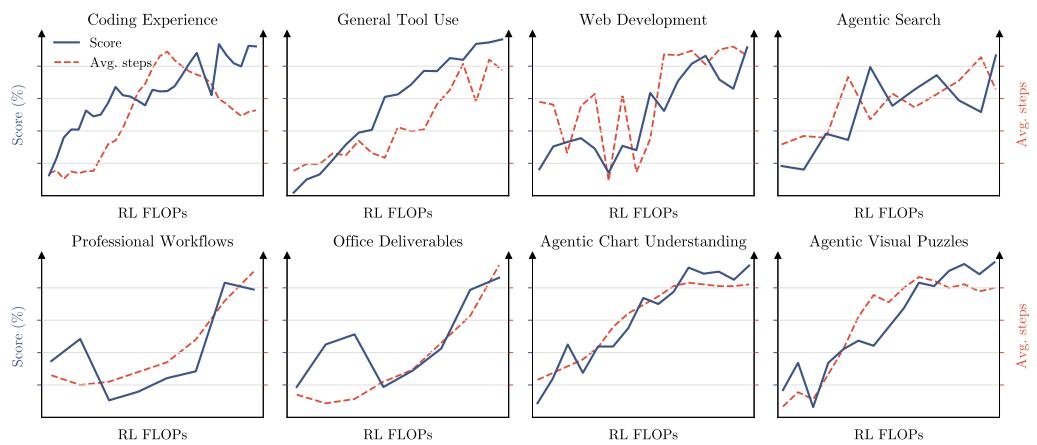
\includegraphics[keepaspectratio,alt={image}]{images/af66c2566cf4e511b94a4eba02991663f913d321e6bad35d3f33e79df573caf2.jpg}}

图 8: RL 过程中各种公开和内部评测的得分与平均助手步数。通过扩展 RL FLOPs，工具调用步数持续增长，同时模型的整体能力得到全面提升。

算法 为缓解在长周期任务中加剧的长尾延迟问题，我们扩展了同步 RL 框架 {[}118, 59{]} 中的部分 rollout 方案。在每次迭代的 rollout 阶段，我们为 N 个提示各采样 K 个补全，保持 \(N \times K\) 个轨迹的活跃工作负载。生成阶段不会等待所有 rollout 终止，而是在比例为 \(\lambda \in ( 0 , 1 )\) 的轨迹完成时（即 \(\lambda N K\) 条）暂停，使策略优化能够继续进行而不受执行掉队者的拖累。暂停的 rollout 被入队并优先在下一次迭代开始时恢复，由我们的沙箱基础设施提供支持（§ 5.3.2）。一旦某个提示的所有 \(\bar { K }\) 个响应完成，它们立即被分派进行策略优化，优化过程遵循 Kimi K2.5 {[}59{]} 中的算法。在我们的部分 rollout 方案下，单条长周期轨迹自然地跨越多次迭代，引入了威胁训练稳定性的数据陈旧性问题。我们的策略优化算法通过逐 token 正则化天然地容忍这种极端的离策略（off-policy）状态。通过将策略更新约束在一个局部邻域内，该正则化使算法能够稳健地处理高度陈旧的数据，并维持训练稳定性。

推理努力 RL 为在最大化 token 效率的同时微调推理努力，我们在 RL 中实现了逐问题的预算控制机制 {[}59{]}。我们为每个问题 x 关联一个由冷启动模型估计的初始 token 预算 \(b _ { 0 } ( x )\)，并将总 token 预算 \(\dot { T } ( y )\) 超过缩放阈值 \(\tau \cdot b _ { 0 } ( x )\) 的轨迹的任务奖励覆盖为 1。对于通用任务，\(T ( y )\) 衡量思考 token 的数量；对于智能体任务，\(T ( y )\) 则计算累积输出 token，包括推理轨迹和工具调用参数。训练遵循围绕预算乘数 τ 的阶段式课程。我们首先训练一个具有相对较大 τ 的最大预算变体，同时仍对最大预算设置上限以抑制过度思考。然后我们将 τ 退火到较小值，以获得高努力和低努力的专家模型。τ 的调整在每个领域内根据人工参与指导进行配置。所有推理级别下由各专家产生的轨迹被统一收集，用于监督微调和多教师在线策略蒸馏。

智能体生成式奖励模型 对于不可验证的通用任务，我们采用智能体生成式奖励模型（GRM），保留了 Kimi K2.5 {[}58, 59{]} 中基于锦标赛风格、使用二值比较的群体奖励方法。除了增强判断所需的通用智能体能力外，智能体评判器还必须遵循一个强制协议：（1）阅读结果、产物或文本输出；（2）生成评分标准（rubric）；（3）对照评分标准给每个候选打分；以及（4）将评分标准分配的分数记录在评分板（scorepad）中。为缓解针对越来越冗长的输出的奖励黑客（reward hacking）行为，我们应用了与上述推理努力控制类似的基于预算的冗长度控制：给定从冷启动模型估计的初始冗长度 \(\ell _ { 0 }\) 和一个乘数 σ，输出长度超过 \(\sigma \cdot \ell _ { 0 }\) 的候选将自动输掉二值比较。

\subsubsection{多教师在线策略蒸馏}\label{multi-teacher-on-policy-distillation}

我们采用多教师在线策略蒸馏（MOPD）将这些在不同推理努力程度下的领域专用能力整合到统一模型中 {[}75, 134, 29{]}。在训练过程中，对于给定的领域 d 和采样的推理努力级别 \(e \in \{ \mathrm { l o w } , \mathrm { h i g h } , \mathrm { m a x } \}\)，优化由九个专家中对应的教师模型 \(\pi _ { \mathrm { t e a c h e r } } ^ { ( d , e ) }\) 引导。给定输入查询 x 和前缀响应 \(y _ { < t }\)，在教师 \(\pi _ { \mathrm { t e a c h e r } } ^ { ( d , e ) }\) 和学生 \(\pi _ { \theta }\) 之间，在 \(y _ { t }\) 上评估的逐 token OPD 奖励定义为：

\[
r _ {\mathrm{opd}} ^ {d} (y _ {t} \mid e, x, y _ {<   t}) = \operatorname{clip} \left(\operatorname{sg} \left(\log \frac {\pi_ {\text {teacher}} ^ {(d , e)} (y _ {t} \mid x , y _ {<   t})}{\pi_ {\theta} (y _ {t} \mid e , x , y _ {<   t})}\right), - R _ {\max}, R _ {\max}\right),\tag{15}
\]

其中 \(\operatorname { s g } ( \cdot )\) 表示停止梯度算子，\(R _ { \operatorname* { m a x } } > 0\) 是用于约束极端优势信号的裁剪阈值，从而稳定 RL 训练。这一密集奖励信号无缝集成到我们的 RL 框架中，自然地支持基础设施级优化，例如针对长周期任务的部分 rollout 训练。虽然我们也实验了更细粒度的 top-k 蒸馏目标，但在我们的设置中，无论是在收敛速度还是最终性能方面，均未观察到明显优势。

\subsubsection{部署感知的后训练}\label{deployment-aware-post-training}

MXFP4 量化感知后训练 为在部署时减少内存占用和服务成本，我们将 MoE 专家权重——这些权重占据了模型参数内存的主要部分——量化到 MXFP4 {[}103{]}，激活值以 MXFP8 计算，而所有非专家组件（注意力投影、潜在 MoE 投影、共享专家和 MoE 路由器）保持更高精度。我们在整个后训练阶段（覆盖 SFT 和 RL）进行量化感知训练（QAT）{[}49{]}，使模型适应量化引入的精度损失。在 RL 过程中，rollout 和训练共享相同的量化方案——消除了训练与推理之间的不匹配。

草稿模型微调 优化推理效率对于服务复杂的、长周期的智能体模型至关重要。Kimi K3 在预训练时带有一个多 token 预测（MTP）层，其结构与主干块镜像。由于 EAGLE-3 {[}71{]} 的草稿模型由结构与 MTP 层匹配的单个解码器层组成，我们将预训练的 MTP 层微调为 EAGLE-3 风格的草稿模型，目标模型冻结，仅更新草稿层及其特征融合投影。遵循 EAGLE-3 的训练时测试协议，草稿在训练期间展开七步；除第一步外——最新位置的目标侧特征不可用——草稿从较早步骤消费自己的输出，镜像了推理时的循环草稿过程。

草稿输入融合了目标模型的低层、中层和高层特征，分别取自第 1、第 4 和最后一个 AttnRes 块的输出 \(( \ S ~ 2 . 2 )\)。这些特征被拼接并通过一个无偏置矩阵 \(W _ { \mathrm { E 3 } }\) 投影到隐藏维度，该矩阵初始化为 \(\left[ \textbf { 0 0 } \pmb { I } \right]\)，使得融合表示在初始化时与高层特征 \(h _ { h }\)——即 MTP 层预训练时的输入——一致，并在微调过程中逐渐学会融入低层和中层特征。

推测解码的加速效果由无损推测采样下的逐 token 接受率 \(\begin{array} { r } { \sum _ { x \in \mathcal { V } } \operatorname* { m i n } ( p ( x ) , q ( x ) ) } \end{array}\) 决定，其中 p 和 q 分别表示目标模型和草稿模型的下一 token 分布。由于最小化传统的 KL 散度代理目标并不能保证对容量有限的草稿模型最大化该接受率，我们直接优化基于似然的 LK 损失 {[}104{]}，即接受率本身的对数负值，

\[
\mathcal {L} _ {\mathrm{LK}} = - \log \sum_ {x \in \mathcal {V}} \min (p (x), q (x)),\tag{16}
\]

其中 p 和 q 在温度 1 下评估，且不包含辅助的真实交叉熵项。草稿微调遵循后训练 QAT 配置 \(( \ S 4 . 1 . 4 )\)，MoE 专家权重采用 MXFP4，其输入激活采用 MXFP8，而非专家模块保持更高精度。

\subsection{RL 任务合成与智能体环境}\label{rl-task-synthesis-and-agentic-environments}

我们的 RL 框架的有效性在很大程度上依赖于丰富、多样且可稳健验证的环境。为支持跨复杂长周期任务的可扩展训练，我们设计了一系列专用的白盒环境和任务合成范式。

\subsubsection{统一白盒 RL 环境}\label{unified-white-box-rl-environment}

使用单一固定的智能体框架（harness）进行训练可能导致模型过拟合到特定的工具模式、系统提示、上下文管理机制或交互协议。为解决此问题，我们开发了一个统一白盒 RL 环境，将智能体框架表示为一组可配置、可组合的模块，包括工具接口、系统提示、上下文管理策略、技能、记忆、子智能体和其他组件。通过配置组合这些模块，该环境可以实例化主流框架，如 Kimi Code {[}56{]}、Claude Code {[}15{]}、Codex {[}20{]}、OpenClaw {[}86{]} 和 Hermes {[}44{]}，以及全新的框架。在 RL 训练过程中，我们为不同的任务组动态构建不同的框架配置，使 Kimi K3 暴露于这些模块的多样化组合，而非任何单一框架的惯例。同样的抽象也方便地支持跨各种任务领域的 RL，为训练更通用的智能体提供了可扩展的基础。

\subsubsection{知识图谱引导的任务合成}\label{knowledge-graph-guided-task-synthesis}

动机与概览 后训练任务的质量和多样性在很大程度上取决于其源材料。由细粒度概念引导的检索能够发掘专业化和未被充分代表的知识，而跨多样化概念的采样则拓宽了领域覆盖范围。为在大规模下同时控制粒度和覆盖范围，我们构建了一个自演化、层次化组织的知识图谱，智能体通过在知识密集型和编码领域的 Web 规模探索持续扩展该图谱。图 9 展示了任务合成流水线。

\pandocbounded{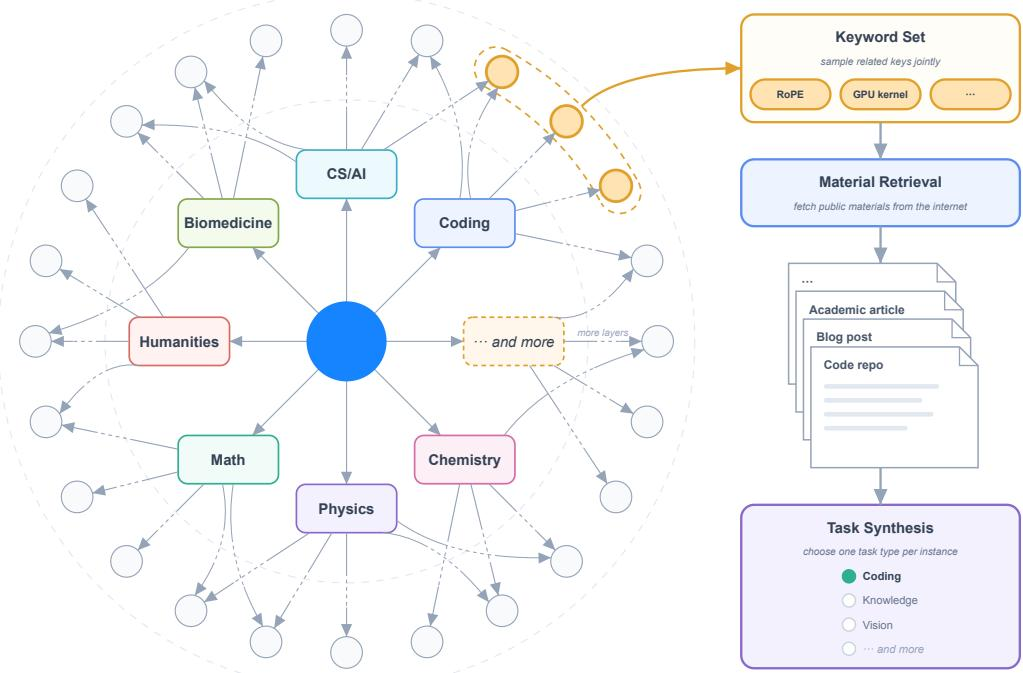
\includegraphics[keepaspectratio,alt={image}]{images/7a620cf00c87d1d5b1eb0f9473a087b6fdbbeca22f1f12c3383e30a860d84b3a.jpg}}

图 9: 知识图谱引导的任务合成概览。层次化组织的知识图谱在多个层级表示概念，范围从广泛领域到细粒度概念。相关节点被采样形成一个关键词集合，引导公开源材料的检索。对于每个合成实例，系统选择一个任务类型，并使用检索到的材料合成相应的任务。

智能体知识图谱构建 我们将知识图谱构建为一个有向无环图，通过递归的、智能体驱动的扩展来实现。扩展过程从一组预定义的粗粒度种子节点开始。每个节点被分配一个智能体实例，该实例执行多次 Web 搜索以调研相应的概念。在添加新节点之前，智能体会探索现有图谱以识别等价或相关的概念，在适当的地方复用已有节点，以最小化重复。边始终从较粗粒度的概念指向较细粒度的概念，无论智能体首先发现哪个端点。新添加的节点随后被分配给智能体进行进一步探索。当分配的智能体确定当前概念已经足够原子化时，该分支停止扩展。

材料检索与任务合成 为针对跨领域和任务类型的期望分布，系统在不同粒度级别采样节点，可以单独采样或按相关组合采样。从采样节点派生的关键词与来自知识图谱中其祖先节点的上下文信息相结合，以生成 Web 查询。检索到的真实世界材料被组合起来，由合成智能体生成各种任务类型的训练任务。

\subsubsection{智能体环境中的可验证问题}\label{verifiable-problems-in-agentic-environments}

我们在智能体环境中训练 Kimi K3 解决可验证问题；代表性示例包括：多步骤复杂信息搜索，其中模型规划研究过程、逐步从 Web 收集证据并产生可验证的答案；专业人士的真实日常工作，如投资银行、数据分析和法律实务，其中模型将复杂请求分解、在沙箱中操作领域工具，并在数十到数百个步骤中完成交付物；以及针对 STEM 问题、视觉谜题和图表理解的多步骤可验证视觉推理。每条视觉推理轨迹在配备 Python 解释器的隔离沙箱智能体环境中生成：模型迭代编写和执行代码来裁剪、缩放或变换输入图像，执行精确计算或验证中间结果，并在多个交互步骤中接收执行输出——包括生成的图像——作为新的观察。随着模型学会执行更多的图像操作并收集更多的观察，其在复杂视觉推理任务上的表现稳步提升。

\subsubsection{内核优化任务}\label{kernel-optimization-tasks}

为增强 Kimi K3 的 GPU 内核优化能力，我们构建了一个大规模内核任务套件，涵盖从单算子内核到融合巨型内核的各种任务，其来源包括诸如 Flash Linear Attention {[}139{]} 等高质量 GitHub 仓库。该套件覆盖了多种 GPU 编程方法，如 CUDA、Triton、CuTe DSL、Gluon、ThunderKittens {[}110{]} 和 TileLang {[}129{]}，并涵盖了广泛使用的 GPU 架构和数值格式，包括 BF16、FP8 和 FP4。奖励同时评估正确性和性能：每个内核提供 PyTorch 参考实现，超出预定义数值误差阈值的解决方案获得零奖励。性能则相对于专家实现进行评分：与之匹敌获得 0.5 奖励，接近硬件理论峰值（roofline）则将奖励提高到接近 1。为确保奖励反映真实的优化，我们开发了一个黑客检测系统，惩罚诸如 CUDA 图重放、输入缓存和精度降低等奖励黑客策略，并在 Kimi K3 开发过程中观察到新的黑客策略时持续扩展新的防护措施。

\subsubsection{个人助理任务}\label{personal-assistant-tasks}

对于长周期个人助理任务，我们开发了广泛使用应用的真实模拟实现，如 Gmail、Notion、Slack 和 Canvas。这些模拟实现保留了其真实对应物的核心语义，同时支持可复现的大规模交互，无需外部 API 或频率限制。在这些模拟应用的基础上，我们设计了受真实世界专业工作流启发的复杂任务，场景涵盖人力资源、法律服务和金融等领域。在每个任务中，智能体在一个持久的、持续演化的环境中运作，跨越多个模拟天数，并遇到分布在各个应用中的数十个相互依赖的事件。单次 rollout 可能涉及多达数千次工具调用和数百万上下文 token。每个事件带有自己的评估标准，由确定性规则或基于 LLM 的评估器评判。初始工作空间由自主搜索 Web 获取参考材料并将其转换为连贯的、与任务相关环境的智能体构建。我们还扩展了 RL 框架以支持此类活环境（living environments），对复杂事件流及其引发的世界状态转换进行建模。

\subsubsection{自主执行任务}\label{autonomous-execution-tasks}

我们引入自主执行任务（AET），这是一种通过验证闭环（verify-in-the-loop）优化训练长周期智能体智能的环境范式。每个任务指定初始状态、受约束的目标、基于工具的动作空间、执行预算以及一个独立的验证器。智能体仅看到目标、上下文、约束和验证接口，没有参考轨迹或预定义流程，必须自主执行任务分解、工具选择、规划、错误恢复和终止。奖励基于验证器对最终环境状态的评估，而非智能体自报的完成情况。我们设计了多种类型的验证器以支持多样化的环境，包括黑盒系统复现（图 10）、量化因子发现和税务审计。在每个环境中，智能体迭代提交解决方案、接收验证器反馈并优化策略，训练其假设、执行、分析反馈和适应的通用循环。通过将智能体与验证器隔离、将提供诊断反馈的公开验证器与评估留出场景的隐藏验证器配对，以及在有限提交预算下施加基于惩罚的奖励，来缓解奖励黑客行为。

\subsubsection{Web 开发任务}\label{web-development-tasks}

我们构建了一个多样化的、由专家精心策划的 Web 开发任务套件，覆盖典型场景。输入范围从单行场景描述到多段落规格说明；产物涵盖网站、交互式游戏、3D/WebGL 场景、数据可视化、SVG 和全栈应用。每个任务在容器化沙箱中运行，并在多样化智能体框架而非单一固定框架下 rollout，以促进跨框架泛化。奖励由两部分组成：确定性检查和由内部奖励模型进行的模型评判。确定性检查对应用行为进行功能测试，并对复现参考物的任务评分结构和像素级相似度。当项目构建失败、运行出错或伪造而非实现产物时，奖励清零。模型评判使用其他模型进行源代码检查，或查看并交互输出产物。

Camera Repair Management System 复现

\pandocbounded{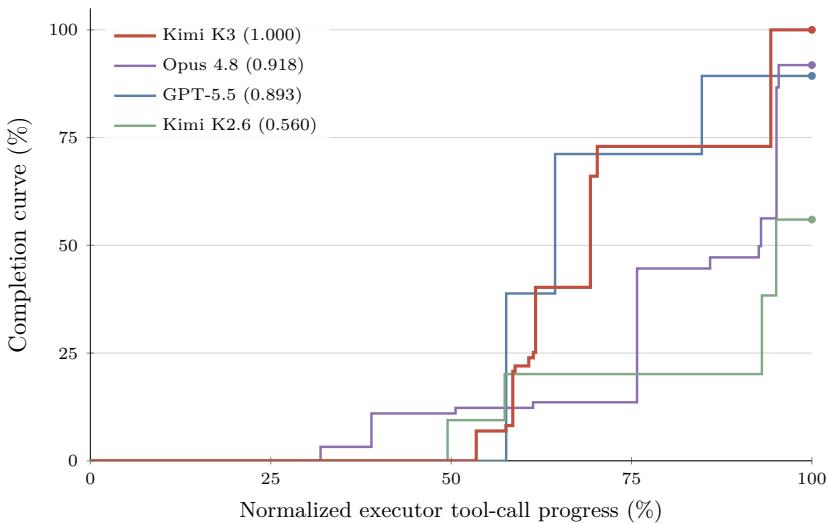
\includegraphics[keepaspectratio,alt={image}]{images/89335c91f0633cd42fe73cb26f193890a1a7be554ff5be446982e23c2739c691.jpg}}

图 10: Camera Repair Management System 上的完成曲线，这是一个黑盒系统复现任务，智能体通过神谕（oracle）查询将一个隐藏的 3D 相机维修系统重建为 Web 应用。完成度表示验证器评估的任务进度。

